

% --------------------------------------------------------------

% This is all preamble stuff that you don't have to worry about.

% Head down to where it says "Start here"

% --------------------------------------------------------------



\documentclass[titlepage]{report}

\usepackage[top=.75in,bottom=.75in,left=0.5in,right=0.5in]{geometry} 
\usepackage{amsmath,amsthm,amssymb,scrextend,mathtools,siunitx, cancel, bm, xfrac, esint}
\usepackage{mdframed}
\usepackage{csquotes}
\usepackage{tabto}
\usepackage{tikz}
\edef\restoreparindent{\parindent=\the\parindent\relax}
\usepackage{parskip}
\restoreparindent
\usepackage[hang,flushmargin,bottom]{footmisc}
\usepackage{longtable}

\usepackage{parskip,caption,gensymb}
\usepackage{graphicx,wrapfig,booktabs,multirow}
\usepackage{multicol}
\usepackage{placeins}
\graphicspath{./}
\usepackage{url}
\usepackage[table,xcdraw,dvipsnames]{}
\usepackage{fancyhdr,color,soul}
\usepackage{tikz}
\usepackage{textgreek}
\usepackage{float}
\usepackage{soul}

\renewcommand{\baselinestretch}{1.5} %this is your line spacing, current at, you guessed it! 1.5
\pagestyle{fancy}


\usepackage[breaklinks=true,hidelinks]{hyperref} %remove [hidelinks] and all links will have box surrounding
\usepackage{changepage}
\usepackage{enotez}

\usepackage{color}

\usepackage{xcolor}
\usepackage[fontsize=12pt]{fontsize}

\definecolor{codegreen}{rgb}{0,0.6,0}
\definecolor{codegray}{rgb}{0.5,0.5,0.5}
%\definecolor{lightgray}{rgb}{0.5,0.5,0.5}
\definecolor{codepurple}{rgb}{0.58,0,0.82}
\definecolor{backcolour}{rgb}{0.95,0.95,0.92}
\definecolor{backcolourt}{rgb}{0.95,0.95,0.92}
\definecolor{quotecolor}{rgb}{211,211,211}
\definecolor{chromeyellow}{rgb}{1.0, 0.65, 0.0}
\definecolor{Highlight}{HTML}{C04F17}
\definecolor{danger}{HTML}{800000}

\usepackage[cache=false]{minted}
\usepackage[most,minted,breakable,skins]{tcolorbox}

\setminted[tasm]{%
	bgcolor=backcolour,
	linenos=true,
	breakanywhere=true,
	labelposition=topline,
	fontfamily=tt,
	fontsize=\footnotesize
}
\usemintedstyle{xcode}

\newtcblisting[number format=\arabic]{code}[2]
{
	listing engine=minted,
	minted language=#1,
	minted options={mathescape, breaklines=true, breakanywhere=true, fontfamily=tt, fontsize=\footnotesize},
	listing only,
	breakable,
	enhanced,
	colback=backcolour!10,
	coltitle=white,  
	title={#2},
}

\tcbset{breakable}

% if you want to define a new color use this format: {name}{RBG}{R, G, B values}
%\definecolor{teal}{RGB}{0, 128, 128 } 
\definecolor{ltgray}{gray}{0.95}

\renewcommand{\thefootnote}{\arabic{footnote}}

\newcommand*{\hamil}{\hat{\mathcal{H}}}


\newcommand{\N}{\mathbb{N}}

\newcommand{\Z}{\mathbb{Z}}

\newcommand{\I}{\mathbb{I}}

\newcommand{\R}{\mathbb{R}}

\newcommand{\Q}{\mathbb{Q}}

\renewcommand{\qed}{}

\let\newproof\proof



\renewenvironment{proof}{\begin{mdframed}[backgroundcolor=ltgray]\begin{addmargin}[1mm]{1mm}\footnotesize\begin{newproof}}{\end{newproof}\end{addmargin}\end{mdframed}\qed}
% \newcommand{\expl}[1]{\text{\hfill[#1]}$}

\newenvironment{theorem}[2][Theorem]{\begin{trivlist}
		
		\item[\hskip \labelsep {\bfseries #1}\hskip \labelsep {\bfseries #2.}]}{\end{trivlist}}


\newenvironment{lemma}[2][Lemma]{\begin{trivlist}
		
		\item[\hskip \labelsep {\bfseries #1}\hskip \labelsep {\bfseries #2.}]}{\end{trivlist}}

\newenvironment{problem}[2][Problem]{\begin{trivlist}
		
		\item[\hskip \labelsep {\bfseries #1}\hskip \labelsep {\bfseries #2.}]}{\end{trivlist}}

\newenvironment{exercise}[2][Exercise]{\begin{trivlist}
		
		\item[\hskip \labelsep {\bfseries #1}\hskip \labelsep {\bfseries #2.}]}{\end{trivlist}}

\newenvironment{reflection}[2][Reflection]{\begin{trivlist}
		
		\item[\hskip \labelsep {\bfseries #1}\hskip \labelsep {\bfseries #2.}]}{\end{trivlist}}

\newenvironment{proposition}[2][Proposition]{\begin{trivlist}
		
		\item[\hskip \labelsep {\bfseries #1}\hskip \labelsep {\bfseries #2.}]}{\end{trivlist}}

\newenvironment{corollary}[2][Corollary]{\begin{trivlist}
		
		\item[\hskip \labelsep {\bfseries #1}\hskip \labelsep {\bfseries #2.}]}{\end{trivlist}}



\newtcolorbox{functionspec}[1]{%
	breakable,
	enhanced,
	borderline north = {.5mm}{0mm}{blue},
	arc=0pt,
	outer arc=0pt,
	colframe=white,
	colback=white,
	coltitle=blue!70!black,
	fonttitle=\ttfamily\normalsize\bfseries,
	fontupper=\ttfamily,
	boxed title style={empty},
	title={#1}}

\usepackage{setspace}
\newtcolorbox{notespec}{
	breakable,
	enhanced,
	frame empty,
	borderline west = {1.5mm}{0mm}{yellow},
	fontlower=\bfseries,
	fontupper=\bfseries,
	colback=white,
	colback=yellow!5
}

\newtcolorbox{warningspec}{
	breakable,
	enhanced,
	frame empty,
	borderline west = {1.5mm}{0mm}{red},
	fontlower=\bfseries,
	fontupper=\bfseries,
	colback=white,
	colback=red!5
}

\newtcolorbox{newquote}{
	fontupper=\normalsize\itshape,
	fontlower=\footnotesize,
	colframe=gray!50,
	boxrule=0.1pt,
	colback=gray!25
}
\setlength{\parindent}{0pt}

\newcommand{\critical}[1]{{\color{danger}\textbf{#1}}}

% --------------------------------------------------------------

%                         Start here

% --------------------------------------------------------------



%\lhead{left}

%\chead{center}

%\rhead{Right}

%If you uncomment any/all of the above, you can set your own headers, uncommenting one will remove the auto headers in place (section and subsection) 


\makeatletter\@enumdepth1\makeatother

\makeatletter
\def\@Aboxed#1&#2&#3\ENDDNE{%
	\ifnum0=`{}\fi \setbox \z@
	\hbox{$\displaystyle#1{}\m@th$\kern\fboxsep \kern\fboxrule }%
	\edef\@tempa {\kern  \wd\z@ &\kern -\the\wd\z@ \fboxsep
		\the\fboxsep \fboxrule \the\fboxrule }\@tempa 
	\fcolorbox{white}{ltgray}{$\displaystyle #1#2$}% changed
}
\makeatother
\begin{document}
	
	\begin{titlepage}
		\begin{center}
			\vspace*{1in}
			{\Large\textbf{lwIP-CE with TLS 1.3\\Whitepaper}}\\
			\vspace*{0.5in}
			{\huge\textbf{Analysis\\\vspace{10px}Justifications}}\\
			\vspace*{1in}
			by Anthony Cagliano
		\end{center}
	\end{titlepage}
	\setcounter{secnumdepth}{2}
	\setcounter{tocdepth}{2}
	\tableofcontents	
	
	\newpage
	\section{Foreword}
	
	
	\textbf{CryptX} is a suite of dynamic libraries designed for use with the LIBLOAD functionality of the C and ez80 Assembly toolchain\footnote{https://github.com/CE-Programming/toolchain} for the TI-84+ CE graphing calculator. The library group provides implementations for many industry-standard cryptographic algorithms enabling developers to securely transmit data between endpoints using their applications. It implements some of the most secure encryption technologies in use today, porting them in a manner that provides modest security while also remaining feasible to run on the calculator.
	
	CryptX is not just another haphazard construction similar to others you might see in the software archives of several calculator programming websites that boasts password storage or the ability to hide or protect files. CryptX is the result of research, coding, and analysis by many individuals within the TI-84+ development community with varying areas of expertise. The project was conceptualized and implemented by a cryptographer \& cybersecurity analyst. Other contributing developers were ez80 assembly experts who assisted in ensuring the efficiency and security of various algorithms (ex: writing in constant-time) or hardware experts who provided information on such things as entropy derivation. I would like to offer a special thanks to the members of the TI programming community, whose support and assistance has made the continuing development of this library possible.
	
	Before we move into the API Documentation, allow me to justify this library's existence against those who will cite the unwritten rule of cryptography--"Don't roll your own crypto". This is valid on platforms where tested and proven solutions for cryptography exist; no such luxury exists on the TI-84+ CE. I began work on CryptX as a proof-of-concept and as a learning exercise in basic encryption. Over time, not only did I begin receiving some positive feedback from the calculator community but I also found that I genuinely enjoyed working on it. I decided to stay the course and do the best I could to turn it into a legitimate cryptography resource for the community. This library isn't a total sin against said unwritten rule, however. Where possible, encryption algorithms are ported from known-good implementations; where not possible, algorithm specifications are presented for peer review (see the \href{sec:analysis}{Cryptanalysis}). Additionally, known weaknesses (particularly those introduced by the nature of the hardware) are documented and steps taken to mitigate them are also presented for peer review.
	
	
	\newpage
	\section{Implementation Overview}
	\label{sec:implementation_overview}
		In this section we review the security profile of CryptX to allow the more technically-minded among our users to appreciate the effort put into making this library as secure as possible. Where necessary, algorithm constructions are documented for peer review. It is also noteworthy that this library is an open-source project. Therefore the entire code base is available on Github\footnote{https://github.com/acagliano/cryptx\\\textit{CryptX source code repository on Github.}}. Additionally, methods used to improve side-channel resistance are also presented for peer review. This section is live-updated as more information becomes available. 
	
	\section {Entropy-Sourcing}
	\label{sec:entropy}
	

	\subsection{Secure RNG Construction \& Analysis}
	\label{ssec:csprng}
	\subsubsection{Rationale \& Difficulties}
	The first question to answer in the quest to devise a secure RNG was: Does the TI-84+ CE produce randomness, and if so, (1) what is the nature of this randomness (does it have entropy?) and (2) how does this differ by hardware revision? The calculator is unlike a computer in that it lacks many of the dynamic sources of entropy that go into generating randomness for those platforms. It was intially intended to use the r register or CPU clock cycle counter, but this was rapidly discarded after the discovery that both of those are predictable. At a loss, and with insufficient knowledge of the device hardware mechanics, I posted on Cemetech seeking information about possible sources of randomness on the TI-84+ CE. Cemetech user \texttt{Zeroko} came to the rescue with data on hardware bus noise.
	\begin{newquote}
		SRAM has a pair of bitlines for each bit of each column address, which are connected to a circuit that tries to make them both be charged to an equal, high level before reading from a memory cell (which partially discharges one of the two) and to a sense amplifier (basically a comparator) to read the resulting state afterward. (There may also be another level of gating between the bitlines and the comparators, but that does not strongly affect the dynamics.) In the unmapped space, there are no memory cells, so the controller equalizes the bitlines however well it does, then does nothing (there being no memory cell to discharge them), then senses which bitline is at a higher level. For some column addresses, this will be heavily biased one way or the other because the pre-charge transistors on the bitlines are too different, while for others, it will be less biased because they are more similar.\footnotemark
	\end{newquote}
	\footnotetext{https://www.cemetech.net/forum/viewtopic.php?p=293079\\\textit{Producing crypto-safe randomness on the TI-84+ CE.}}
	\subsubsection{Source-Selection Algorithm}
	Based on statistical analysis of the unmapped space, it became clear that there was a very large subset of possible source bytes that appeared entropic and that these subsets differed by hardware revision. After some discussion an algorithm was constructed (with optimization support from Adam Beckingham) that would poll each byte in the unmapped space 1024 times and then count the deviation.
	
	As the algorithm proceeds through the unmapped space, it maintains an internal pointer to the most entropic source it has encountered as well as a value to beat on the degree of deviation. If the algorithm encounters a better source, it updates the internal pointer and the value to beat. By the time the algorithm finishes polling the unmapped space, it will have selected the best possible source of entropy. That source address is retained by the library for use gathering entropy and cannot be modified by the user.
	
	Should the algorithm fail to find a suitable source (the maximum allowable bias is 75\%/25\% in either direction), the initialization function will return FALSE.
	
	\subsubsection{Entropy-Gathering Algorithm \& Mitigating Correlation}
	The RNG internally reserves an entropy pool 119 bytes large in the device’s accelerated RAM. 119 bytes was chosen because it fits nicely within two (2) SHA-256 blocks. To generate a random number, each byte in the entropy pool is updated by reading from the selected source byte. The entire pool is then passed through the SHA-256 cryptographic hash, generating a 32-byte digest. That hash is broken into 8-byte blocks, each byte of which is XORed together to produce a single byte. The result is a 4-byte compression of the 119-byte entropy pool.
	
	Due to the nature of the CE hardware, there is a measurable correlation in the values of floating bits within unmapped memory. This correlation varies depending on the sample size, but would measurably reduce the entropy of the system. While specific numbers on the degree of correlation are, as of yet, unavailable, we do know that there are higher amounts of correlation in the initial reads which decreases after a certain number of reads. Zeroko provided a more technical explanation of this as well.
	\begin{newquote}
		Another source of non-randomness distinct from the bias is that the bitlines act like capacitors, so precharging only moves their voltage toward the desired level rather than reaching it. This results in a correlation between reads, with the correlation getting weaker with a longer time interval between them and with more intervening reads performed. This is why we cannot just use a von Neumann extractor (which only de-biases) and instead have to do something like XORing many consecutive bits together (which does not fully remove the bias and correlation but can lower it to an undetectable level).  \footnotemark
	\end{newquote}
	\footnotetext{https://www.cemetech.net/forum/viewtopic.php?p=293079\\\textit{Producing crypto-safe randomness on the TI-84+ CE.}}
	To solve this problem, Zeroko performed some analysis on the unmapped memory and revealed that XORing seven (7) reads together per byte would be sufficient to trend the actual entropy closer to what is calculated above.
	
	
	\subsubsection{Proof of Cryptographic Strength}
	
	In order to be secure (at least on paper), a PRNG has to pass 2 distinct additional unpredictability assessments in addition to the requirement that it also pass general statistical randomness tests (which this generator does for sufficient sample sizes). The two additional tests are the \textbf{next-bit test} and the \textbf{state compromise test}\footnote{https://en.wikipedia.org/wiki/Cryptographically\_secure\_pseudorandom\_number\_generator\\\textit{Reference on basic requirements for CSRNG.}}.\\\\
	\ul{Next-Bit Test}
	\begin{addmargin}[1em]{1em}
		The \textit{Next-Bit Test} is defined as follows: given the prior output of the PRNG, the next bit of the output cannot be predicted by a polynomial-time statistical test with a probability non-negligibly greater than 50\%.
		
		To prove this we need to evaluate the entropy of the selected source. As the entropy varies depending on what bit is selected, we will compute the entropy of the worst-case to keep things simple and take that as the \textbf{minimum} effective entropy of the generator. The worst-case is the set of probabilities $P = \{0.75, 0.25\}$. This means that a bit will be set 75\% of the time and reset the rest of the time or vice versa.\\
		
		\begin{proof}
			\textbf{Mathematical Entropy Demonstrations on Worst-Possible Entropy Tap}
			
			Assumptions:\\
			The worst possible bias will be 75/25 on a bit (guaranteed by generator behavior).\\
			The only bounded entropy source in this proof is the worst-possible bit.\\
			We assume zero entropy for any other bit in a byte read.\\
			We read from the entropy source in XOR mode 7 times per byte into a 119 byte entropy pool.\\
			
			To model min-entropy while mapping read-to-read correlation without introducing a full dependence model, we use an effective sample count:
			\[
			n_{\text{eff}}=\max\!\left(1,\left\lfloor\frac{n}{k}\right\rfloor\right)
			\]
			where:\\
			$k$ is a correlation factor\\
			($k=1$ means independent reads, $k=7$ means fully correlated over the 7-read XOR window).\\
			I presented this way because we do not currently have a number we can rely on for $k$.
			
			Using $p=0.75$ and $n=7$:
			\[
			p_{\oplus}(k)=\frac{1-(1-2p)^{n_{\text{eff}}}}{2}
			\]
			\[
			p_{\oplus}(1)=0.5039,\qquad p_{\oplus}(7)=0.75
			\]
			\[
			H_{\infty}(k)=-\log_2\!\left(\max\!\left(p_{\oplus}(k),1-p_{\oplus}(k)\right)\right)
			\]
			\[
			H_{\infty}(1)=0.9888,\qquad H_{\infty}(7)=0.4150
			\]
			
				\begin{figure}[H]
					\centering
					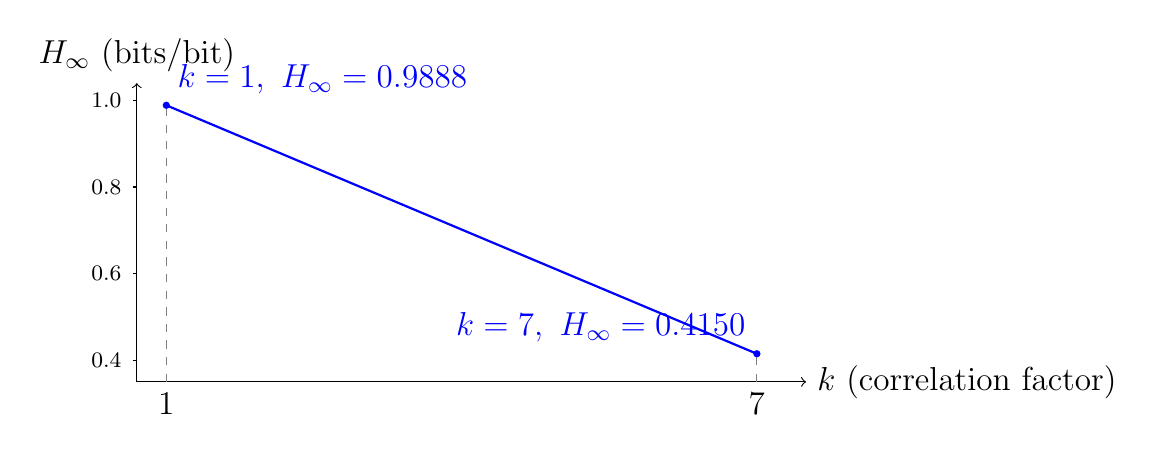
\begin{tikzpicture}[x=1.25cm,y=5.5cm]
					\draw[->] (0.7,0.35) -- (7.5,0.35) node[right] {$k$ (correlation factor)};
					\draw[->] (0.7,0.35) -- (0.7,1.04) node[above] {$H_{\infty}$ (bits/bit)};
					\foreach \yy/\lbl in {0.4/0.4,0.6/0.6,0.8/0.8,1.0/1.0}
					{
						\draw (0.66,\yy) -- (0.7,\yy);
						\node[left] at (0.66,\yy) {\scriptsize \lbl};
					}
					\draw[dashed,gray] (1,0.35) -- (1,0.9888);
					\draw[dashed,gray] (7,0.35) -- (7,0.4150);
					\draw[thick,blue] (1,0.9888) -- (7,0.4150);
					\filldraw[blue] (1,0.9888) circle (1.1pt) node[above right] {$k=1,\ H_{\infty}=0.9888$};
					\filldraw[blue] (7,0.4150) circle (1.1pt) node[above left] {$k=7,\ H_{\infty}=0.4150$};
						\node[below] at (1,0.35) {$1$};
						\node[below] at (7,0.35) {$7$};
					\end{tikzpicture}
					\vspace{0.6em}
					\caption{Correlation sensitivity for 7-read XOR whitening (endpoint model $k\in\{1,7\}$).}
				\end{figure}
				
				For the full entropy pool (119 bytes), we use:
				\[
				H_{\infty,\text{pool}}(k)=119\cdot H_{\infty}(k)
				\]
				\[
				H_{\infty,\text{pool}}(1)=117.6672,\qquad H_{\infty,\text{pool}}(7)=49.3850
				\]
				
				\begin{figure}[H]
					\centering
					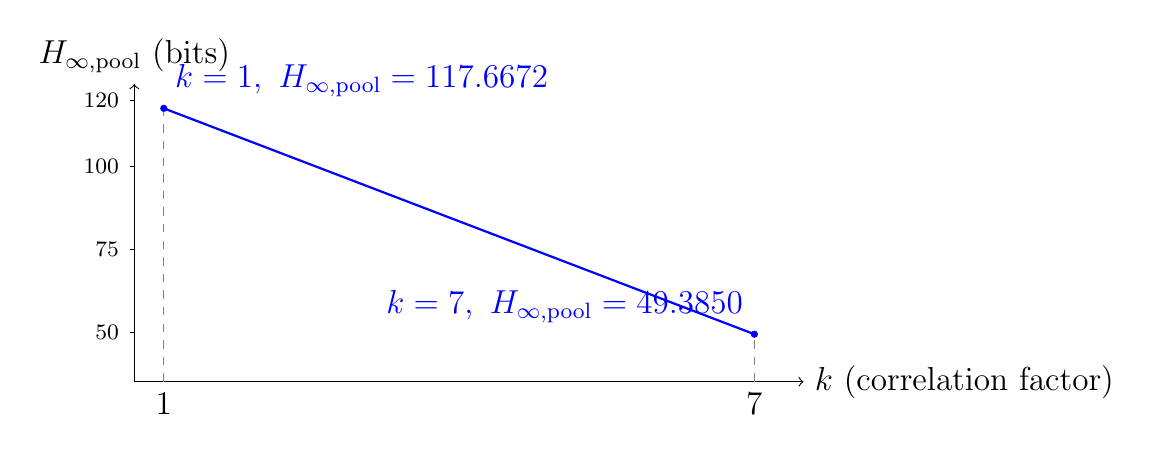
\begin{tikzpicture}[x=1.25cm,y=0.042cm]
						\draw[->] (0.7,35) -- (7.5,35) node[right] {$k$ (correlation factor)};
						\draw[->] (0.7,35) -- (0.7,125) node[above] {$H_{\infty,\text{pool}}$ (bits)};
						\foreach \yy/\lbl in {50/50,75/75,100/100,120/120}
						{
							\draw (0.66,\yy) -- (0.7,\yy);
							\node[left] at (0.66,\yy) {\scriptsize \lbl};
						}
						\draw[dashed,gray] (1,35) -- (1,117.6672);
						\draw[dashed,gray] (7,35) -- (7,49.3850);
						\draw[thick,blue] (1,117.6672) -- (7,49.3850);
						\filldraw[blue] (1,117.6672) circle (1.1pt) node[above right] {$k=1,\ H_{\infty,\text{pool}}=117.6672$};
						\filldraw[blue] (7,49.3850) circle (1.1pt) node[above left] {$k=7,\ H_{\infty,\text{pool}}=49.3850$};
						\node[below] at (1,35) {$1$};
						\node[below] at (7,35) {$7$};
					\end{tikzpicture}
					\vspace{0.6em}
					\caption{Correlation sensitivity for whole-pool min-entropy (119-byte pool, endpoint model $k\in\{1,7\}$).}
				\end{figure}
				
				Under the conservative correlation model used here, the generator still produces sufficient min-entropy per 32-bit output block, including the worst-case endpoint (k=7). In that sense, the construction is mathematically adequate on paper for the stated security target.
				
				However, this section is a model-based argument, not a certification result. It does not by itself prove real-world security. Actual security also depends on hardware behavior, implementation correctness, side-channel resistance, and empirical validation on target devices.
				
				Therefore, these proofs should be read as theoretical lower-bound reasoning, complemented by continuous testing and external review, not as a standalone assurance of cryptographic safety.
		\end{proof}
		\footnotetext{https://tsapps.nist.gov/publication/get\_pdf.cfm?pub\_id=915121\\\textit{Entropy requirements for secrets and nonces.}}
		
	\end{addmargin}
	\ul{State Compromise Test}
	\begin{addmargin}[1em]{1em}
		The \textit{State Compromise Test} simply means that an adversary that somehow gains knowledge of the generator's state remains unable to predict its output. This means that deterministic generators that have their outputs influenced by some seed value are not suitable for cryptography unless the output incorporates sufficient entropy.
		
		The RNG in CryptX does not use a seed value at all, instead relying entirely on entropy for its output. The only state it maintains is the byte initially selected as the source of entropy. However, because the source has sufficient entropy, an attacker who knows what bit is being used to gather entropy still should be unable to reconstruct the output stream with probability non-negligibly higher than 50\% per bit of output.
		
		Another consideration is \textit{runtime state manipulation}. The TI-84+ CE is not a multitasking-capable processor, therefore the device can only process one code path at a time. This removes vulnerability to local state manipulation (changes to state by other code running on the device). Additionally, the library halts system interrupts while the random number generation code is running, which halts system USB activity. This renders state manipulation via that method impossible as well.
	\end{addmargin}
	
	The previous stated, I assert that the output of the generator satisfies all algorithmic constraints for cryptographic security and is thus safe for use as a cryptographic RNG.
	
	\critical{Note that these proofs only apply to physical hardware (an actual TI-84+ CE), not to emulators.} Due to the inability of an emulator to accurately reproduce the behavior of the unmapped region, they implement a deterministic RNG to create the illusion of randomness for that range of memory. This yields statistical randomness with an obscurity factor due to how CryptX selects the source, but the randomness is still not cryptographically secure. Bear this in mind when using CryptX from an emulator.
	
	\subsection{Side-Channel Analysis}
	CryptX has an unknown level of resistance to side-channel analysis. The TI-84+ CE is not a device constructed with true hardware security in mind. After all it is just a calculator and I'm sure that when it was being designed no-one anticipated the level of awesome but ridiculous nonsense the TI programming community would one day achieve. However, when it did become a reality, and the security of their calculators was called into question by a video showcasing an exam mode exploit, rather than taking practical steps to resolve the issue (which would have included a code analysis/vulnerability review leading to the inevitable discovery that the exploit in question was patched two TI-OS versions ago), Texas Instruments' resolution was instead to unnecessarily disable ez80 assembly code execution (and not even do it properly). This angered the entire programming community, which includes people skilled enough to find and leak other vulnerabilities. Part of cybersecurity is limiting your attack surface and that includes understanding the risk inherent in doing dumb things that make people more keen to breach your security. It is in that aspect of risk management (as well as other areas) that TI demonstrably fails. Because let me remind us once more that \critical{bad security is often worse than no security at all}.
	
	With that rant over, let's circle back to the subject matter at hand -- CryptX's resistance to side-channel analysis. There are very limited ways in which a device designed to be plugged into a computer and memory-mapped can be protected against being plugged into a computer and memory-mapped. That being said, I took some actions that could reasonably be taken without slowing down the library's functions to harden it against these types of attacks.
	
	\subsubsection{Timing Analysis Resistance}
	One of the first considerations in this library was resistance to timing analysis, but this is particularly difficult on this platform as everything takes longer, which multiplies out deviations in execution time that may be indistinguishable on faster platforms. Additionally all code is CPU only; there are no dedicated chips that can be easily accessed that may implement some form of hardware timing control. While I have not as of the time of this writing evaluated the ported functions, all functions written from scratch for this platform had this form of hardness in mind and are constant time to the best extent possible. Here is an overview of what is known at present.
	\begin{itemize}
		\item\textbf{SRNG generation}: Timing analysis leaks number of 32-bit blocks generated, but not precise length or value.
		\item\textbf{cryptx\_digest\_compare}: Written from scratch by \texttt{jacobly} and uses an algorithm that defeats timing analysis.
		\item\textbf{AES CBC mode}: Timing analysis leaks number of blocks encrypted, but not precise data length.
		\item\textbf{AES CTR/GCM modes}: Timing analysis leaks precise data length.
		\item\textbf{RSA/powmod}: Written from scratch for speed by \texttt{jacobly} and is resistant to timing analysis if run from normal speed memory.
		\item\textbf{ECDH}: Written in assembly, underlying arithmetic constant-time in all places possible.
	\end{itemize}
	
	\subsubsection{Buffer Leak Protection}
	Another consideration taken is to avoid leaving residual computational data in the stack frame after a function that performs data transformations completes. For this reason, some code was written that purges the stack frame and we call that code in most of the user-facing encryptor functions before returning control to the caller. For reference, the code used to accomplish this is:
	\inputminted{tasm}{code/stack_clear.asm}
	\subsubsection{Memory-Mapping Protection}
	After resolving buffer leaks, our attention turned to thwarting attempts to map the device's memory while sensitive operations are running to gain information about the encryption or decryption. While there is sufficient difficulty in achieving this on this device, I believe the solution arrived at is sufficient.
	
	It is the system interrupt that makes it possible for the operating system to handle activity on the USB port, and disabling said interrupts would severely hamper attempts to read CryptX's operating state by preventing the system from responding to USB activity. For this reason, some code was written that disables interrupts in all functions where data is being encrypted or decrypted, or nonces are being generated, saving the previous interrupt state to SMC, and restoring that state afterwards. While there are many variations of this code that operate in slightly different ways depending on when they are called, here is the basic version of it, for reference:
	\inputminted{tasm}{code/disable_interrupts.asm}
	
	\subsection{Algorithmic Security}
	\subsubsection{CPA Resistance}
	CPA is an acronym for \textit{chosen plaintext attack}, a type of attack against a cipher that involves manipulating the encryption algorithm to reveal session information. A simple description of this attack is that by requesting multiple encryptions of the same plaintext, but each time changing a bit of the input, you can begin to reveal bits of the session key used to encrypt it.
	
	The cipher modes that are strong against this particular form of attack, most notably CBC, CTR, GCM, OCB, EAX (in essence everything except ECB), prevent it through the inclusion of a nonce -- a string of random bytes -- that is incorporated into the encryption, turning the deterministic blockwise encryption into a psuedo-random permutation. This means that even if you encrypt the exact same plaintext with no modification, each output will be different. This eliminates an attackers ability to leak session information in this manner.
	
	CryptX provides CBC, CTR, and GCM modes, all of which are randomized encryption algorithms and thus provide security against chosen plaintext analysis.
	\subsubsection{CCA Resistance}
	CCA is an acronym for \textit{chosen ciphertext attack}, a type of attack against a cipher that involves an attacker manipulating the decryption algorithm to reveal session information. The objective of the attacker is the same as in CPA, to reveal the session key by observing how the plaintext responds to manipulation of bits in the ciphertext. Nonce inclusion does not help us here because the nonce is known to the algorithm used for decryption and is part of the metadata used to decrypt. Defense against CCA requires \textit{authenticated encryption} which is a combination of encryption with data integrity verification.
	
	There are two ways to accomplish CCA properly:
	\begin{itemize}
		\item\textbf{Encrypt then hash or HMAC}\\This method involves using a standard CPA-resistant cipher mode to encrypt the plaintext and then to pass the nonce, ciphertext, and any additional data (ex: headers) to a hash or HMAC algorithm to generate an authentication tag. Send the nonce, additional data, ciphertext, and tag to the other party for decryption. That party should verify that the hash or HMAC they compute matches the one you sent BEFORE decrypting the message. Should the validation fail, the message should be refused without decryption.
		\item\textbf{Authenticating cipher mode}\\This method involves using a specialized cipher mode such as GCM, GCM-SIV, OCB, or EAX that incorporates authentication as part of the encryption. Many of these algorithms use a mathematical construction that is secure within the context of the session (such as Galois field multiplication over a hash key derived from the encryption key) so long as you ensure proper nonce handling. These cipher modes allow additional authenticated data (AAD) and generate an authentication tag that should be sent to the other party along with the encrypted message. The other party should validate the tag and reject the message without decrypting if the tag they compute does not match the one you sent.
	\end{itemize}
	
	CryptX provides an API for using either method and they are secure as long as any constraints specified within the documentation are followed.
	\subsection{Conclusion}
	In summation, CryptX is a work in progress and sees regular updates that add resistance to various forms of attack. While its algorithmic security is solid if implemented properly, there are weaknesses in the hardware of the device that make a full security evaluation of the library difficult. For this reason, use CryptX only for low-risk applications...logging in to game servers, custom secure services for calculators, and similar. You should not be sending anything requiring true security using a calculator.
	
	If you have any questions about the proper usage of CryptX in your programs, any of its functionality, algorithms, etc, please do not hesitate to contact me on Discord at \texttt{acagliano\#3685}. I would rather you ask questions than implement security improperly and risk compromising your implementation. I also enjoy discussing and learning about cybersecurity in general.
	
	{\color{red}\textbf{Please update to new stable releases as soon as they become available and update any software you are developing to use the latest versions of HASHLIB as soon as you are able. At this stage in development, updates are usually security enhancements, not major feature additions.}}
	
	Special thanks to the following individuals who contributed materially to the project:
	\begin{singlespace}
		\begin{tabular}{l | p{12cm}}
			\textbf{Lead Developer} & Anthony Cagliano\\\hline
			\textbf{C $\rightarrow$ EZ80} & Adam Beckingham\\\hline
			\textbf{Code Contributions} & John Caesarz\newline jacobly\newline Zeroko\newline calc84maniac\\\hline
			\textbf{Info \& Analysis} & Zeroko\newline MateoC: "That's not how you implement RSA, you idiot."\\\hline
			\textbf{QA \& Testing} & placeholder
		\end{tabular}
	\end{singlespace}
	\newpage
	\subsection{Other References}\small
	\begin{enumerate}
		\item[1] \ul{https://github.com/B-Con/crypto-algorithms/}\\\textit{Source of ported AES and SHA-256 algorithms.}
		
		\item[2] \ul{https://github.com/kokke/tiny-ECDH-c}\\\textit{Source of reference ECDH implementation.}
		
		\item[4] \ul{https://datatracker.ietf.org/doc/html/rfc4868}\\\textit{SHA-256 HMAC implementation details.}
		
		\item[5] \ul{https://nvlpubs.nist.gov/nistpubs/Legacy/SP/nistspecialpublication800-38d.pdf}\\\textit{AES-GCM implementation details.}
		
		\item[6] \ul{Modern Cryptography and Elliptic Curves, A Beginner's Guide}, Thomas R. Shemanske.\\
		\textit{Reference for learning elliptic curves.}
	\end{enumerate}
	
	\subsection{Legal}\small
	This software is released under the terms of the \textbf{GNU General Public License Agreement v3.0}. To sum a stupidly long document into something short enough that people might actually read it: You can do whatever you want with the source code to this project so long as you don't stop anyone else from doing whatever they want with it. What does this mean? You can use the source code in your own stuff (called \textit{derived work}) in all or in part or even modified but you cannot supersede the open source license on derived components, pursue claims of infringement against other developers for their own utilization of our code, or pursue liability claims against this project for your use of our code\footnote{https://www.gnu.org/licenses/gpl-3.0.en.html}. 
	
	
\end{document} 
